\documentclass[12pt,letterpaper]{article}           % fleqn: align equations left

% Document:
\usepackage{geometry}                                     % Custom margins for single page, etc.
\usepackage{fullpage}                                     % Use the full page
\usepackage{setspace}                                     % Enables custom margins, doublespacing, etc.
\usepackage{pdflscape}                                    % Use: \begin{landscape} ... \end{landscape}

% Font/text:
\usepackage[latin9]{inputenc}                             % Font definition and input type
\usepackage[T1]{fontenc}                                  % Font output type
\usepackage{lmodern}                                      % Latin Modern fonts
\usepackage{textcomp}                                     % Supports many additional symbols

%\usepackage[urw-garamond]{mathdesign} %dont use with amssymb, etc
%%%%Packages used without Mathdesign
\usepackage{amsmath}                                      % Math equations, etc.
\usepackage{amsthm}                                       % Math theorems, etc.
\usepackage{amsfonts}                                     % Math fonts (e.g. script fonts)
\usepackage{amssymb}                                      % Math symbols such as infinity
\DeclareMathOperator*{\Max}{Max}                          % Better looking max function
\DeclareMathOperator*{\Min}{Min}                          % Better looking min function

%%%%%%%%%%%%%%%%%%%%%%%5
\usepackage{xcolor}                                        % Enables colored text
\definecolor{darkblue}{rgb}{0.0,0.0,0.66}                 % Custom color: dark blue
\usepackage[hyperfootnotes=false,bookmarksopen]{hyperref} % Enable hyperlinks, expand menu subtree
\hypersetup{                                              % Custom hyperlink settings
    pdffitwindow=false,                                   % true: window fit to page when opened
    pdfstartview={XYZ null null 1.00},                    % Fits the default zoom of the page to 100%
    pdfnewwindow=true,                                    % Links in new window
    colorlinks=true,                                      % false: boxed links; true: colored links
    linkcolor=darkblue,                                   % Color of internal links
    citecolor=darkblue,                                   % Color of links to bibliography
    urlcolor=darkblue  }                                  % Color of external links

% Images:
\usepackage{graphicx}                                     % Allows .jpg images to be included
%\usepackage{epstopdf}                                    % Convert .eps images on the fly
%\usepackage{subfig}                                       % Enables arrayed images
\usepackage[section]{placeins}                            % Forces floats to stay in section
\usepackage{float}                                        % Used with restylefloat
\restylefloat{figure}                                     % "H" forces a figure to be "exactly here"
\usepackage[justification=centering]{caption}             % Center captions
\usepackage{subfig} %allow multiple floats in a figure



%\usepackage{datetime}                                     % Custom date format for date field
%\newdateformat{mydate}{\monthname[\THEMONTH] \THEYEAR}    % Defining month year date format
\usepackage{tikz}                                        % Timelines and other drawings
\usetikzlibrary{decorations}                             % Formating for Tikz
\usetikzlibrary{calc}
\usetikzlibrary{matrix}
\usetikzlibrary{positioning}
\definecolor{darkred}{rgb}{0.8,0,0}
\usepackage{tikz-3dplot}


%%%%%%%%%%%%%%%%For Filling in the area between to curves
\usepackage{pgfplots}
\pgfplotsset{compat=1.11}
\usepgfplotslibrary{fillbetween}
\usetikzlibrary{intersections}
\usetikzlibrary{patterns}
\usepgfplotslibrary{ternary}


\pgfdeclarelayer{bg}
\pgfsetlayers{bg,main}

%%%%%%%%%%%MATH
\usepackage{graphicx}
\usepackage{caption}
%\usepackage{subcaption} %this produces an error with the package subfig

%Flow Chart
\tikzstyle{decision} = [diamond, draw, fill=blue!20, text width=4.5em, text badly centered, node distance=3cm, inner sep=0pt]
\tikzstyle{block}    = [rectangle, draw, fill=black!25, text width=5em, text centered, rounded corners, minimum height=4em]
\tikzstyle{line}     = [draw, -latex']
\tikzstyle{cloud}    = [draw, ellipse,fill=red!20, node distance=3cm, minimum height=2em]

\pagestyle{empty}

%%%%%%%%%%%%%%%%%%%%%%%%%%%%%%%5
\begin{document}


	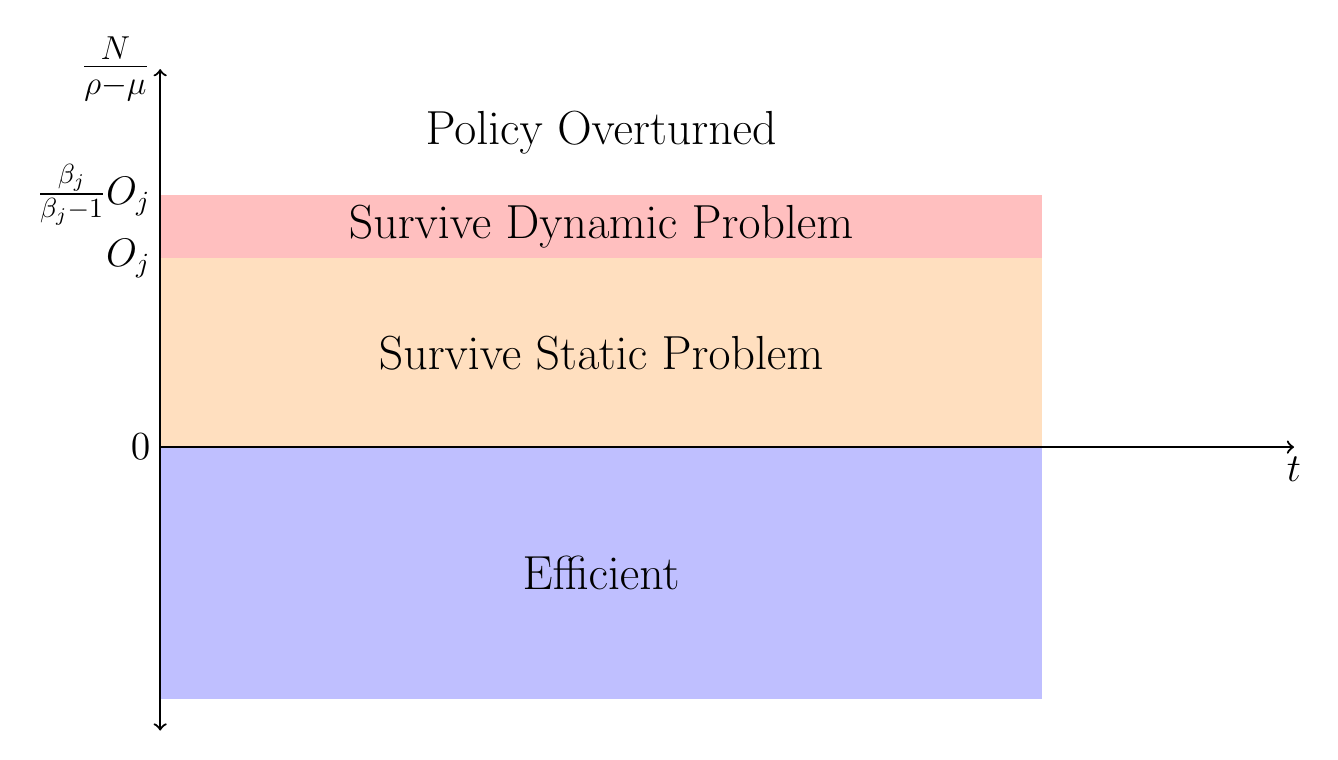
\begin{tikzpicture}[scale=0.8]
	
	\node [left] at (0, 0) {\Large{$0$}};
	\fill [blue,nearly transparent] (0,0) rectangle (14,-4);
	
	\node [left] at (0, 3) {\Large{$O_j$}};
	\fill [orange,nearly transparent] (0,0) rectangle (14,3);
	
	\node [left] at (0, 4) {\Large{$\frac{\beta_j}{\beta_j - 1}O_j$}};
	\fill [red,nearly transparent] (0,3) rectangle (14,4);
	
	\draw [thick] [->] (0,0)--(18,0) node[right, below] {\Large{$t$}};
	
	\draw [thick] [<->] (0,-4.5)--(0,6) node[above, left] {\LARGE{$\frac{N}{\rho - \mu}$}};
	
	\node [] at (7,-2) {\LARGE{Efficient}};
	\node [] at (7,1.5) {\LARGE{Survive Static Problem}};
	\node [] at (7,3.5) {\LARGE{Survive Dynamic Problem}};
	\node [] at (7,5) {\LARGE{Policy Overturned}};
	
	\end{tikzpicture}


\newpage

	  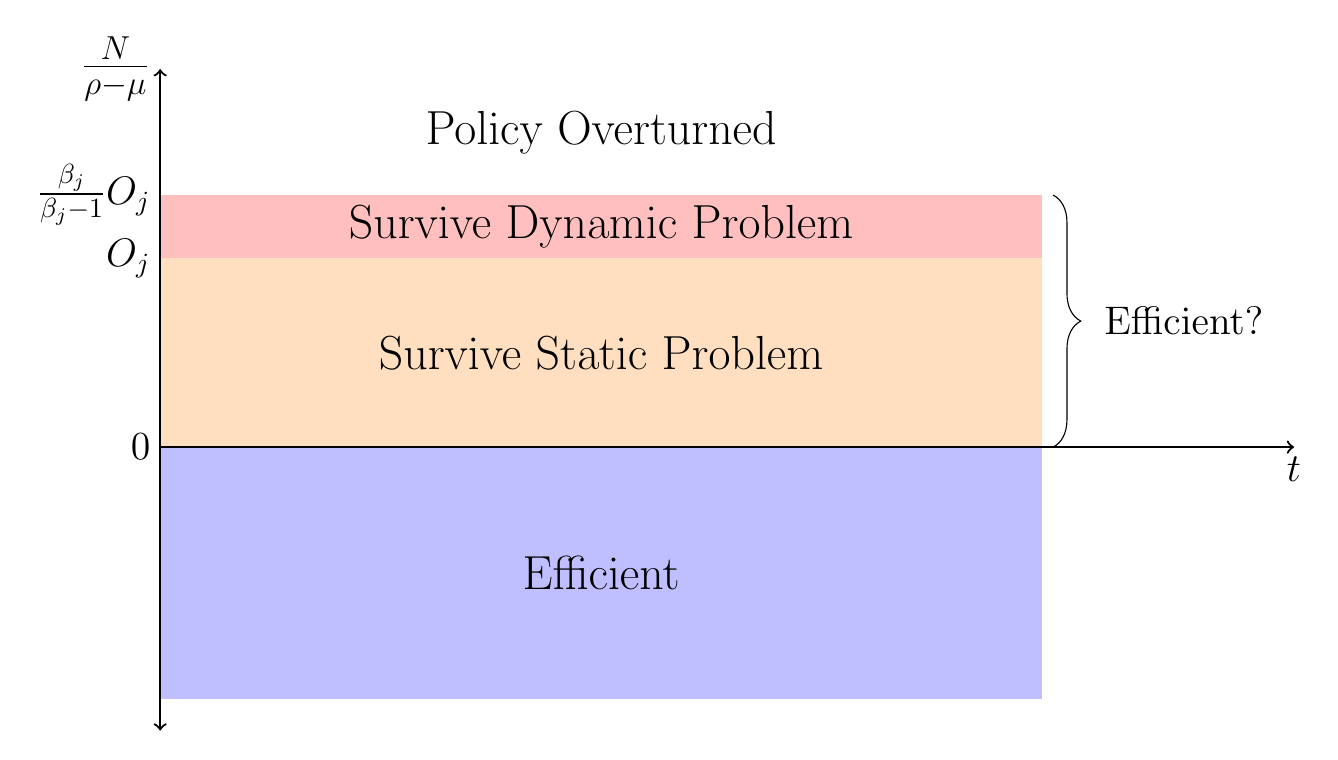
\begin{tikzpicture}[scale=0.8]
	
	\node [left] at (0, 0) {\Large{$0$}};
	\fill [blue,nearly transparent] (0,0) rectangle (14,-4);
	
	\node [left] at (0, 3) {\Large{$O_j$}};
	\fill [orange,nearly transparent] (0,0) rectangle (14,3);
	
	\node [left] at (0, 4) {\Large{$\frac{\beta_j}{\beta_j - 1}O_j$}};
	\fill [red,nearly transparent] (0,3) rectangle (14,4);
	
	\draw [thick] [->] (0,0)--(18,0) node[right, below] {\Large{$t$}};
	
	\draw [thick] [<->] (0,-4.5)--(0,6) node[above, left] {\LARGE{$\frac{N}{\rho - \mu}$}};

	\node [] at (7,-2) {\LARGE{Efficient}};
	\node [] at (7,1.5) {\LARGE{Survive Static Problem}};
	\node [] at (7,3.5) {\LARGE{Survive Dynamic Problem}};
	\node [] at (7,5) {\LARGE{Policy Overturned}};
	
	\draw [decorate,decoration={brace,amplitude=10pt,mirror,raise=4pt},yshift=0pt]
	(14,0) -- (14,4) node [black,midway,xshift=1.8cm] {\Large{Efficient?}};
	\end{tikzpicture}


\end{document}
